\PassOptionsToPackage{sorting=none}{biblatex}
\documentclass[
  bibliography=totoc,     % Literatur im Inhaltsverzeichnis
  captions=tableheading,  % Tabellenüberschriften
  titlepage=firstiscover, % Titelseite ist Deckblatt
]{scrartcl}

% Paket float verbessern
\usepackage{scrhack}

% Warnung, falls nochmal kompiliert werden muss
\usepackage[aux]{rerunfilecheck}

% unverzichtbare Mathe-Befehle
\usepackage{amsmath}
% viele Mathe-Symbole
\usepackage{amssymb}
% Erweiterungen für amsmath
\usepackage{mathtools}

% Fonteinstellungen
\usepackage{fontspec}
% Latin Modern Fonts werden automatisch geladen
% Alternativ zum Beispiel:
%\setromanfont{Libertinus Serif}
%\setsansfont{Libertinus Sans}
%\setmonofont{Libertinus Mono}

% Wenn man andere Schriftarten gesetzt hat,
% sollte man das Seiten-Layout neu berechnen lassen
\recalctypearea{}

% deutsche Spracheinstellungen
\usepackage[ngerman]{babel}


\usepackage[
  math-style=ISO,    % ┐
  bold-style=ISO,    % │
  sans-style=italic, % │ ISO-Standard folgen
  nabla=upright,     % │
  partial=upright,   % ┘
  warnings-off={           % ┐
    mathtools-colon,       % │ unnötige Warnungen ausschalten
    mathtools-overbracket, % │
  },                       % ┘
]{unicode-math}

% traditionelle Fonts für Mathematik
\setmathfont{Latin Modern Math}
% Alternativ zum Beispiel:
%\setmathfont{Libertinus Math}

\setmathfont{XITS Math}[range={scr, bfscr}]
\setmathfont{XITS Math}[range={cal, bfcal}, StylisticSet=1]

% Zahlen und Einheiten
\usepackage[
  locale=DE,                   % deutsche Einstellungen
  separate-uncertainty=true,   % immer Unsicherheit mit \pm
  per-mode=symbol-or-fraction, % / in inline math, fraction in display math
]{siunitx}

% chemische Formeln
\usepackage[
  version=4,
  math-greek=default, % ┐ mit unicode-math zusammenarbeiten
  text-greek=default, % ┘
]{mhchem}

% richtige Anführungszeichen
\usepackage[autostyle]{csquotes}

% schöne Brüche im Text
\usepackage{xfrac}

% Standardplatzierung für Floats einstellen
\usepackage{float}
\floatplacement{figure}{htbp}
\floatplacement{table}{htbp}

% Floats innerhalb einer Section halten
\usepackage[
  section, % Floats innerhalb der Section halten
  below,   % unterhalb der Section aber auf der selben Seite ist ok
]{placeins}

% Seite drehen für breite Tabellen: landscape Umgebung
\usepackage{pdflscape}

% Captions schöner machen.
\usepackage[
  labelfont=bf,        % Tabelle x: Abbildung y: ist jetzt fett
  font=small,          % Schrift etwas kleiner als Dokument
  width=0.9\textwidth, % maximale Breite einer Caption schmaler
]{caption}
% subfigure, subtable, subref
\usepackage{subcaption}

% Grafiken können eingebunden werden
\usepackage{graphicx}

% schöne Tabellen
\usepackage{booktabs}

% Verbesserungen am Schriftbild
\usepackage{microtype}

% Literaturverzeichnis
\usepackage[
  backend=biber,
]{biblatex}
% Quellendatenbank
\addbibresource{lit.bib}
% \addbibresource{programme.bib}

% Hyperlinks im Dokument
\usepackage[
  german,
  unicode,        % Unicode in PDF-Attributen erlauben
  pdfusetitle,    % Titel, Autoren und Datum als PDF-Attribute
  pdfcreator={},  % ┐ PDF-Attribute säubern
  pdfproducer={}, % ┘
]{hyperref}
% erweiterte Bookmarks im PDF
\usepackage{bookmark}

% Trennung von Wörtern mit Strichen
\usepackage[shortcuts]{extdash}

% Um Tabellen-Inhalte einzulesen
\makeatletter\let\expandableinput\@@input\makeatother

\KOMAoption{parskip}{half}

\author{%
  Katharina Popp\\%
  \href{mailto:katharina.popp@tu-dortmund.de}{katharina.popp@tu-dortmund.de}%
  \and%
  Nicolai Weitkemper\\%
  \href{mailto:nicolai.weitkemper@tu-dortmund.de}{nicolai.weitkemper@tu-dortmund.de}%
}
\publishers{TU Dortmund – Fakultät Physik}


\subject{V18}
\title{Hochreine Germaniumdetektoren in der Gamma-Spektrometrie}
\date{
    Durchführung: 28.11.2022
     \hspace{3em}
    Abgabe: 17.01.2023
}
\begin{document}

\maketitle
\thispagestyle{empty}
\tableofcontents
\newpage

\section{Zielsetzung}

    Im folgenden Versuch sollen die Spektren verschiedener $\gamma$-Strahler bezüglich ihrer Energie und Aktivität ausgemessen werden.
    Dazu wird ein Germaniumdetektor verwendet,
    welcher zunächst kalibiert und auf seine Vollnachweiswahrscheinlichkeit getestet wird.

\section{Theorie}
\label{sec:theorie}

    Im folgenden Abschnitt werden die theoretischen Grundlagen für diesen Versuch erläutert werden.
    Dabei wird zum einen die Wechselwirkung von Gamma-Strahlung mit Materie,
    sowie die Detektion der Strahlung beschrieben.

\subsection{Wechselwirkung von Gamma-Strahlung mit Materie}

    Gamma-Strahlung besteht aus hochenergetischen Photonen die bei Zerfallsprozessen erzeugt werden.
    In diesem Fall wird der Zerfall des radioaktiven Zerfalls $^{137}\ce{Cs}$ betrachtet,
    welches über einen $\beta$-Zerfall und anschließenden $\gamma$-Zerfall in das stabile $^{137}\ce{Ba}$ zerfällt.
    Dabei wird Strahlung der Energie $E_{\symup{\gamma}} \approx \SI{662}{\kilo\eV}$ \cite{caesium} frei.
    Dieser Prozess ist in \autoref{} dargestellt.
    %\begin{figure}
    %    \centering
    %    \includegraphics[width=\textwidth]{}
    %    \caption{Zerfallsprozess von $^{137}\ce{Cs}$ in das stabile $^{137}\ce{Ba}$. \cite{caesium}}
    %    \label{fig:theorie:zerfallsprozess}
    %\end{figure}

    Wenn die $\gamma$-Strahlung nun auf Materie trifft,
    muss abhängig von der Energie der Strahlung zwischen folgenden Effekten unterschieden werden \cite{radioaktivitaet}.
    Für niedrigere Energien (\%Bereich aus KET) findet größtenteils \textit{Photoeffekt} statt.
    Dabei muss die Energie des Photons $E_{\symup{\gamma}} = hf$ der Bindungsenergie eines der Hüllenelektronen entsprechen.
    Das Photon gibt in diesem Fall seine gesamte Energie an das Elektron ab,
    welches aus dem Atom herausgelöst wird.
    Das Elektron behält dabei eine Energie $E_{e} = hf - E_\text{Bind}$.
    Der Wirkungsquerschnitt unterscheidet sich dabei,
    ob die Energie des Photons kleiner oder größer der relativstischen Ruheenergie des Elektrons ist.
    Es gilt
    \begin{equation*}
        \sigma_\text{Photo} \propto
        \begin{cases}
            \sfrac{Z^5}{E^{\sfrac{7}{2}}_{\symup{\gamma}}} & , E_{\symup{\gamma}} \ll m_{e} c^2 \\
            \sfrac{Z^5}{E_{\symup{\gamma}}} & , E_{\symup{\gamma}} \gg m_{e} c^2 \\
        \end{cases} \ .
    \end{equation*}
    Für zunehmende Energien dominiert der \textit{Compton-Effekt}.
    Das Photon gibt in diesem Fall nicht mehr seine gesamte Energie ab,
    sondern stößt elastisch mit lose gebundenen oder freien Elektronen.
    Dabei gilt Energie- und Impulserhaltung,
    sodass das Photon einen Teil seiner Energie an das Elektron abgibt und beide eine Richtungsänderung erfahren.
    Für den Wirkungsquerschnitt gilt
    \begin{equation*}
        \sigma_\text{Compton} \propto \sfrac{Z}{E_{\symup{\gamma}}} \ .
    \end{equation*}
    Für eine Energie $E_{\symup{\gamma}} \geq 2m_{e}c^2 = \SI{1.022}{\mega\eV}$ kann \textit{Paarerzeugung} stattfinden.
    Dabei wandelt sich das Photon im Coulombfeld des Atoms in ein Elektron-Positron-Paar um.
    Dieser Prozess kann aufgrund der Erhaltungssätze nur mit dem Atomkern als weiteren Stoßpartner stattfinden.
    Die entstehenden Teilchen haben eine Energie von $E_{e^{+}} + E_{e^{-}} = E_{\symup{\gamma}} - 2m_{e}c^2$.
    Weiterhin gilt
    \begin{equation*}
        \sigma_\text{Paar} = Z^2 \ln(E_{\symup{\gamma}}) \ .
    \end{equation*}

    In jedem der Fälle wird die Gamma-Strahlung vom Material absorbiert.


\clearpage

\section{Durchführung}
\label{sec:durchfuehrung}

    Im Folgenden sollen nun der Aufbau des Experiments,
    sowie die Durchführung beschrieben werden.

\subsection{Versuchsaufbau}

    Der Gesamtaufbau besteht zum einen aus einer Rubidium-Spektrallampe,
    welche Licht auf einen Kolben mit Rubidium-Gas strahlt,
    wobei der Kolben von Helmholtzspulen umgeben ist,
    welche verschiedene Magnetfelder erzeugen.
    Das entstehende emittierte Licht wird von einer Photozelle detektiert.
    \autoref{fig:aufbau} zeigt den Aufbau der Apparatur.
    \begin{figure}
        \centering
        \includegraphics[width=\textwidth]{content/img/Abb_1.pdf}
        \caption{Versuchsaufbau mit Spektrallampe, optischen Elementen, Gaskolben und Photoelement. \cite{versuchsanleitung}}
        \label{fig:aufbau}
    \end{figure}

    Wie in \autoref{sec:optisches_pumpen} erläutert,
    soll nun rechts polarisiertes Licht mit der Wellenlänge des $D_1$-Übergangs verwendet werden.
    Dazu sind optische Elemente wie Linsen,
    Polarisationsfilter und beschichtete Plättchen gegeben.
    Mithilfe von plan-konkaven Sammellinsen soll der entstehende Lichtstrahl fokussiert werden.
    Da die Rubidium-Lampe nicht nur die $D_1$-Linie erzeugt,
    werden alle anderen mithilfe eines beschichteten Plättchens herausgefiltert.
    Anschließend wird der Lichtstrahl mithilfe eines Polarisationsfilters erst linear,
    dann mithilfe eines $\sfrac{\lambda}{4}$-Plättchens zirkular polarisiert.

    Mithilfe eines Ofens wird das Rubidium in der Dampfzelle auf einem optimalen Druck gehalten.

    Es wird zwischen verschiedenen Spulen unterschieden,
    welche sich um die Dampfzelle herum befinden;
    eine vertikale Spule und eine horizontale Spule,
    wobei letztere mit einer weiteren Sweep-Spule umwickelt ist.
    Mithilfe der Sweep-Spule können in einer festen Zeit periodisch verschiedene Magnetfeldstärken durchlaufen werden.
    Das Magnetfeld dieser Spulen ist über den Stromfluss regelbar.
    Zusätzlich ist eine Modulationsspule eingebaut,
    welche ein radio-frequentiges Magnetfeld erzeugt,
    dessen Stärke über die Frequenz verstellbar ist.

    Mithilfe eines Oszilloskops kann die registrierte Lichtintensität
    in Abhängigkeit vom Magnetfeld der Sweep-Spule (\textit{XY-Modus})
    dargestellt werden.

\subsection{Einjustierung und Kompensation des Erdmagnetfelds}

    Zu Beginn müssen die optischen Elemente im Strahlengang so justiert werden,
    dass die gemessene Intensität maximal wird.
    Es werden dazu erst die beiden Linsen nacheinander in horizontaler und vertikaler Richtung ausgerichtet
    und anschließend die verschiedenen Filter eingebaut.

    Auf dem Oszilloskop ist nun ein breiter negativer Peak zu sehen.
    Als nächstes muss die Vertikalkomponente des Erdmagnetfelds kompensiert werden.
    Dazu wird der Stromfluss durch die Vertikalspule so erhöht,
    dass der Peak möglichst schmal wird.

    Um die Horizontalkomponente zu kompensieren,
    wird der Tisch, auf dem die Apparatur steht, so gedreht,
    dass der Strahlengang in Nord-Süd-Richtung ausgerichtet ist.
    Auch hier soll der Peak möglichst schmal werden.

\subsection{Messung der Magnetfeldstärke der Rubidium-Isotope}

    Für diese Messung wird das erste Mal ein Strom durch die Modulationsspule gegeben,
    welcher sinusförmig ist und eine Frequenz $f$ hat.
    Die Frequenz wird in der folgenden Messung von \SI{100}{\kilo\hertz} an in Schritten von \SI{100}{\kilo\hertz} bis auf \SI{100}{\mega\hertz} erhöht.

    Beim Anlegen einer Frequenz von \SI{100}{\kilo\hertz} ergibt sich eine Darstellung wie in \autoref{fig:peaks},
    welche während der Messung aufgenommen wurde.
    %\begin{figure}
    %    \centering
    %    \includegraphics[width=\textwidth]{}
    %    \caption{}
    %    \label{fig:peaks}
    %\end{figure}

    Der größte Peak entspricht $B = 0$,
    dort beginnt der Sweep.
    Die beiden kleineren Peaks rechts davon stellen die Rubidium-Isotope dar,
    welche aufgrund des Sweeps symmetrisch um den Null-Peak sind.
    Es ist ausreichend nur auf einer Seite zu messen.

    Das Oszilloskop wird nun so eingestellt,
    dass mit Erhöhen der Stromstärke in der horizontalen Sweep-Spule der Verlauf der Kurve abgelaufen werden kann,
    wobei jeweils der Stromwert notiert wird,
    für den die Spitze eines der Isotopen-Peaks erreicht wird.
    Sollte die Feldstärke der Sweep-Spule nicht ausreichen,
    kann zur Darstellung der Peaks die Stromstärke in der horizontalen Spule erhöht werden.
    Der Gesamtwert der entsprechenden Stromstärke ergibt sich aus Summation der Werte aus beiden Spulen.
    Diese Messung wird für jede Frequenz aus dem oben genannten Bereich wiederholt.

    Zuletzt wird für eine Frequenz von \SI{100}{\kilo\hertz} die Amplitude der beiden Isotopen-Peaks auf dem Oszilloskop vermessen.

\clearpage

\section{Auswertung}
\label{sec:auswertung}

\subsection{Stabilitätsbedingung}
\label{sec:auswertung:stabilitaetsbedingung}
% Aufgabe 2 in der Versuchsanleitung

In \autoref{sec:stabilitaet} wurde anhand der \hyperref[eqn:stabilitaetsbedingung]{Stabilitätsbedingung} die maximale theoretische Resonatorlänge berechnet.
Um diese experimentell zu überprüfen,
wird die Intensität des Lasers für verschiedene Resonatorlängen und Spiegelkonfigurationen gemessen.
\autoref{fig:plt:stabilitaetsbedingung} stellt diese Messwerte dar; die zugrundeliegenden Daten sind in \autoref{tab:stabilitaetsbedingung} aufgeführt.
% In \autoref{fig:plt:stabilitaetsbedingung} sind diese Messwerte dargestellt.

Es ist zu beachten, dass diejenigen Resonatorlängen, bei denen kein Lasern einsetzte, nicht angegeben sind.
Andererseits waren aufgrund der begrenzten Länge der optischen Bank keine größeren Resonatorlängen als etwa \SI{212.8}{\centi\meter} möglich.

\begin{figure}
  \centering
   \includegraphics[width=\textwidth]{build/plt/2_stabilitaetsbedingung.pdf}
   \caption{Lichtintensität $I$ in Abhängigkeit der Resonatorlänge $L$ für verschiedene Spiegelkonfigurationen.}
   \label{fig:plt:stabilitaetsbedingung}
\end{figure}

\begin{table}
\centering
\caption{Messwerte zur Lichtintensität $I$ in Abhängigkeit der Resonatorlänge $L$ für verschiedene Spiegelkonfigurationen.}
\label{tab:stabilitaetsbedingung}
\begin{subtable}{.5\textwidth}
    \centering
    \caption{\enquote{konkav + konkav}}
    \expandableinput{build/tab/2_stabilitaetsbedingung_konkav_konkav.tex}
\end{subtable}%
\begin{subtable}{.5\textwidth}
    \centering
    \caption{\enquote{plan + konkav}}
    \expandableinput{build/tab/2_stabilitaetsbedingung_plan_konkav.tex}
\end{subtable}
\end{table}


% TODO: Mit Theorie-Abschnitt vereinigen
% Durch Lösen von \autoref{eqn:TODO} können die theoretisch größtmöglichen Resonatorlängen $L$ bestimmt werden.
% Hierbei ist zu beachten, dass bei Gleichheit nur noch ein metastabiler Zustand vorliegt.
% \begin{align*}
%     L_\text{max, kk, theo} &= r_1 + r_2 \\
%     L_\text{max, pk, theo} &= r_2 \\
% \end{align*}


\subsection{TEM-Moden}
\label{sec:auswertung:tem_moden}
% Aufgabe TODO in der Versuchsanleitung

\subsubsection{\TEM{00}-Mode}
Die Lichtintensität der \TEM{00}-Mode wird (bei Betrachtung senkrecht zur Strahlachse) durch eine Gauß-Funktion beschrieben.
Um die gemessene Intensitätsverteilung sinnvoll mit der theoretischen zu vergleichen,
werden dabei zusätzliche Parameter für Hintergrund und Verschiebung der Strahlachse eingesetzt.
Daraus ergibt sich \autoref{eqn:tem00_fitfn},
deren Parameter mithilfe von \scipycurvefit an die Messwerte angepasst werden.
\autoref{fig:plt:tem_00} stellt Messwerte und Theoriekurve grafisch dar;
die zugrundeliegenden Daten sind in \autoref{tab:mess_tem_00} aufgeführt.

\begin{equation}
  I =
  I_\text{max} \cdot \exp \left( \frac{-(r - r_0)^2}{2ω^2} \right) + I_0
  \label{eqn:tem00_fitfn}
\end{equation}


Es ergeben sich die folgenden Parameter:
\begin{align*}
  I_\text{max} &= \SI{131.5 \pm 1.1}{\micro\watt}
  \tag{maximale Intensität}
  \\
  I_0 &= \SI{1.7 \pm 0.5}{\micro\watt}
  \tag{Hintergrund, beispielsweise durch Streulicht}
  \\
  r_0 &= \SI{0.082 \pm 0.018}{\milli\meter}
  \tag{Mittelpunkt des Laserstrahls} % bzw. Verschiebung von Strahlachse
  \\
  ω &= \SI{1.968 \pm 0.021}{\milli\meter} % Vorzeichen ist irrelevant!
  \tag{Breite der Gauß-Verteilung}
  \\
\end{align*}

\begin{figure}
  \centering
   \includegraphics[width=\textwidth]{build/plt/3_tem_00.pdf}
   \caption{Lichtintensität $I$ in Abhängigkeit der Distanz $r$ zur optischen Achse für die \TEM{00}-Mode.}
   \label{fig:plt:tem_00}
\end{figure}


\subsubsection{\TEM{01}-Mode}
Die Lichtintensität der \TEM{01}-Mode wird (bei Betrachtung senkrecht zur Strahlachse) durch \autoref{eqn:tem01_fitfn} beschrieben,
wenn wie zuvor zusätzliche Parameter für Hintergrund und Verschiebung der Strahlachse eingesetzt werden.
Das Anpassen der Parameter an die Messwerte erfolgt erneut mit \scipycurvefit.
\autoref{fig:plt:tem_01} stellt Messwerte und Theoriekurve grafisch dar;
die zugrundeliegenden Daten sind in \autoref{tab:mess_tem_01} aufgeführt.

\begin{equation}
  I =
  I_\text{max} \cdot
  \frac{4(r - r_0)^2}{ω^2} \cdot
  \exp \left( \frac{-(r - r_0)^2}{2ω^2} \right) + I_0
  \label{eqn:tem01_fitfn}
\end{equation}

Es ergeben sich die folgenden Parameter:
\begin{align*}
  I_\text{max} &= \SI{3.10 \pm 0.08}{\micro\watt}
  \tag{maximale Intensität}
  \\
  I_0 &= \SI{1.13 \pm 0.09}{\micro\watt}
  \tag{Hintergrund, beispielsweise durch Streulicht}
  \\
  r_0 &= \SI{0.304 \pm 0.024}{\milli\meter}
  \tag{Mittelpunkt des Laserstrahls} % bzw. Verschiebung von Strahlachse
  \\
  ω &= \SI{1.141 \pm 0.017}{\milli\meter} % Vorzeichen ist irrelevant!
  \tag{Breite der Gauß-Verteilung}
  \\
\end{align*}

\begin{figure}
  \centering
   \includegraphics[width=\textwidth]{build/plt/3_tem_01.pdf}
   \caption{Lichtintensität $I$ in Abhängigkeit der Distanz $r$ zur optischen Achse für die \TEM{01}-Mode.}
   \label{fig:plt:tem_01}
\end{figure}

% --- für TEM00 und TEM01 ↓
\begin{table}[H]
\centering
\caption{Messwerte zur Lichtintensität in Abhängigkeit der Distanz zur optischen Achse für verschiedene \TEM{}-Moden.}
\label{tab:mess_tem}
\begin{subtable}{.5\textwidth}
    \centering
    \caption{\TEM{00}}
    \label{tab:mess_tem_00}
    \expandableinput{build/tab/3_tem_00.tex}
\end{subtable}%
\begin{subtable}{.5\textwidth}
    \centering
    \caption{\TEM{01}}
    \label{tab:mess_tem_01}
    \expandableinput{build/tab/3_tem_01.tex}
\end{subtable}
\end{table}


\subsection{Polarisation}
Wie in \autoref{sec:versuchsaufbau} beschrieben,
ist eine nahezu vollständige p-Polarisation des Laserlichts zu erwarten.
Um diese Erwartung zu überprüfen,
wird die Lichtintensität in Abhängigkeit von der Ausrichtung eines Polarisationsfilters gemessen.

Eine theoretische Beschreibung ist durch \autoref{eqn:polarisation_fitfn} gegeben,
%TODO: Ist „Nullwinkel“ überhaupt ein Wort?
wenn zusätzliche Parameter für Hintergrund und Verschiebung des Nullwinkels eingesetzt werden.
Das Anpassen der Parameter an die Messwerte erfolgt erneut mit \scipycurvefit.
\autoref{fig:plt:polarisation} stellt Messwerte und Theoriekurve grafisch dar;
die zugrundeliegenden Daten sind in \autoref{tab:mess_polarisation} aufgeführt.

Es ergeben sich die folgenden Parameter:
\begin{align*}
  I_\text{max} &= \SI{860 \pm 1}{\micro\watt}
  \tag{maximale Intensität}
  \\
  I_0 &= \SI{-6 \pm 8}{\micro\watt}
  \tag{Hintergrund, beispielsweise durch Streulicht}
  \\
  \alpha_0 &= \SI{0.5 \pm 0.4}{\milli\meter}
  \tag{Nullwinkel}
  \\
\end{align*}

\begin{equation}
  I =
  I_\text{max} \cdot \sin(\alpha + \alpha_0)^2 + I_0
  \label{eqn:polarisation_fitfn}
\end{equation}



\begin{figure}
  \centering
   \includegraphics[width=\textwidth]{build/plt/4_polarisation.pdf}
   \caption{Lichtintensität $I$ in Abhängigkeit der Winkeleinstellung $\alpha$ des Polarisationsfilters.}
   \label{fig:plt:polarisation}
\end{figure}

\begin{table}
  \centering
  \caption{Messwerte zur Lichtintensität $I$ in Abhängigkeit des Polarisationswinkels $\alpha$.}
  \label{tab:mess_polarisation}
  \expandableinput{build/tab/4_polarisation.tex}
\end{table}


\FloatBarrier %TODO: nicht mehr nötig, sobald header_common aktualisiert ist!
\subsection{Multimodenbetrieb und Frequenzspektrum des Lasers}
% \subsection{Longitudinale Moden}
% 5. Multimodenbetrieb und Frequenzspektrum des Lasers
Für $L = \SI{162.9}{\centi\meter}$ wird mithilfe eines Oszilloskops das Frequenzspektrum des Lasers im Multimodenbetrieb ausgemessen,
wie in \autoref{fig:screenshot_oszilloskop} gezeigt.
Die ermittelten Peaks sind in \autoref{tab:mess_frequenzspektrum} angegeben.

\begin{figure}
  \centering
   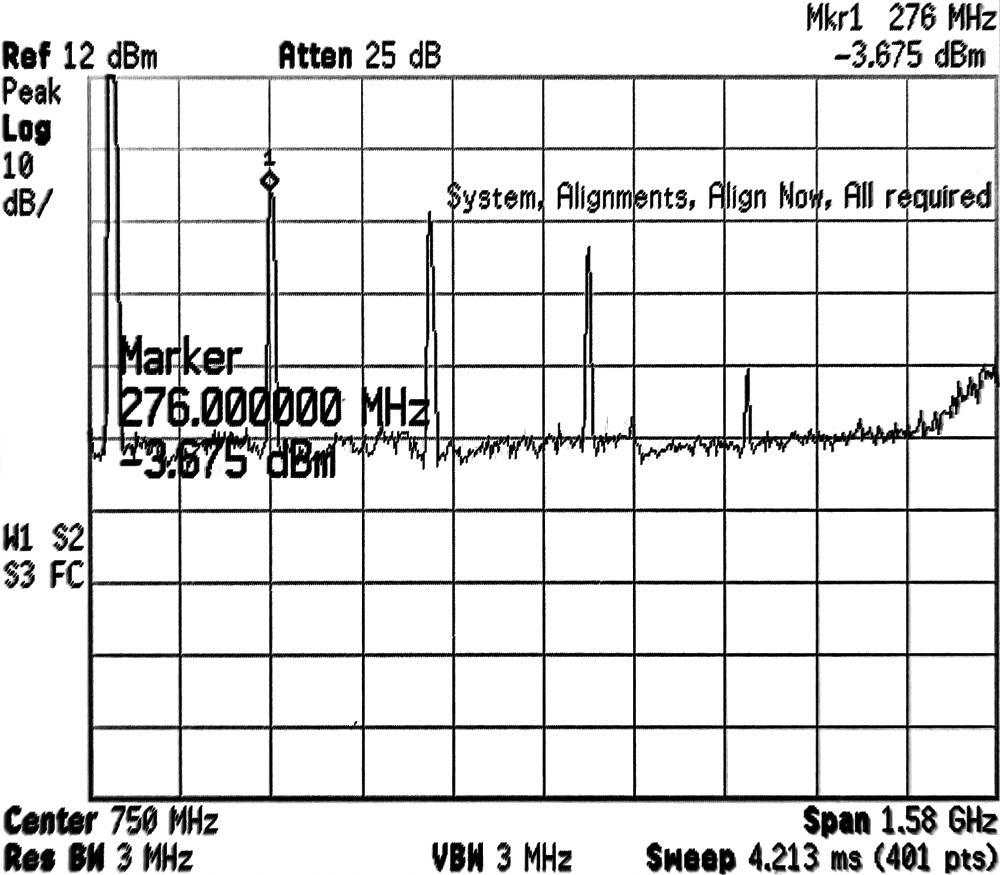
\includegraphics[width=0.75\textwidth]{content/img/5_frequenzspektrum_oszilloskop_inverted.jpg}
   \caption{Bildschirmaufnahme des Oszilloskops.}
   \label{fig:screenshot_oszilloskop}
\end{figure}

\begin{table}
  \centering
  \caption{Messwerte zu den Peaks im Frequenzspektrum. $f$ bezeichnet die Frequenz, $I$ die Intensität.}
  % Intensität hier in dBm=Decibelmilliwatt
  \def\belmilliwatt{Bm} %TODO
  \label{tab:mess_frequenzspektrum}
  \expandableinput{build/tab/5_frequenzspektrum.tex}
\end{table}



\subsection{Wellenlänge}
\label{sec:auswertung:wellenlaenge}
Um die Wellenlänge des Laserlichts zu bestimmen,
werden dessen Beugungsmaxima an verschiedenen optischen Gittern vermessen.

Durch Umformen von
\begin{equation*}
  k \lambda = d \sin(\alpha_k)
\end{equation*}
ergibt sich die praktisch anwendbare Bestimmungsgleichung
\begin{equation}
  \lambda = \frac{d a_k}{k \sqrt{e^2 + a_k^2}} \ ,
  \label{eqn:wellenlaenge}
\end{equation}
wobei $k$ die Ordnung des Beugungsmaximums,
$d$ der Spaltabstand (Gitterkonstante),
$e$ der Abstand zwischen Gitter und Schirm, % Oxford-Komma: Persönliche Präferenz, eigentlich nicht richtig.
und $a_k$ der Abstand des Beugungsmaximums zum Hauptmaximum (und somit zur optischen Achse)
ist.

Die Messwerte, anhand derer die Wellenlänge nun bestimmt wird, sind in \autoref{tab:mess_wellenlaenge} zu finden.
Dort sind auch die nach \autoref{eqn:wellenlaenge} bestimmten Wellenlängen für jede Messreihe angegeben.
% TODO ↓
Im Mittel ergibt sich $\bar\lambda = \SI{12345}{\micro\meter}$.

% Die Ordnung $k$ ist natürlich nicht wirklich vorzeichenbehaftet.
% TODO: In der Tabelle Vorzeichen streichen?

\begin{table}
  \centering
  \caption{
    Abstände der Interferenzmaxima der Ordnung $k$ vom Hauptmaximum für verschiedene optische Gitter.
    Zusätzlich sind der Spaltabstand (inverse Gitterkonstante) $\sfrac{1}{d}$, der Abstand zum Schirm $e$ und die jeweils berechnete Wellenlänge $\lambda$ angegeben.
  }
  \label{tab:mess_wellenlaenge}
  \begin{tabular}{S S S S S}
  \toprule
  & \multicolumn{4}{c}{$\sfrac{1}{d} \mathbin{/} \si{\per\milli\meter}$} \\
  \cmidrule(lr){2-5}
  & 80 & 100 & 600 & 1200 \\
  \midrule

  & \multicolumn{4}{c}{$e \mathbin{/} \si{\centi\meter}$} \\
  \cmidrule(lr){2-5}
  & 90.5 & 90.5 & 63.0 & 33.0 \\
  \midrule

  {$k$} &
  \multicolumn{4}{c}{$a_k \mathbin{/} \si{\centi\meter}$} \\
  \midrule

  \expandableinput{build/tab/6_wellenlaenge.tex}
  \midrule

  & \multicolumn{4}{c}{$\lambda \mathbin{/} \si{\nano\meter}$} \\
  \cmidrule(lr){2-5}
  & 460.05 \pm 5.46 & 643.74 \pm 7.53 & 641.60 \pm 7.96 & 328.51 \pm 16.07 \\
  \bottomrule
  \end{tabular}
\end{table}

\clearpage

\section{Diskussion}
\label{sec:diskussion}

\subsection{Abweichungen}
Bei der \hyperref[sec:auswertung:koinzidenz]{Justage der Koinzidenzapparatur} zeigte sich
ein Maximum der Zählrate bei einer kleinen Zeitverschiebung
und davon ausgehend ein symmetrischer, weitestgehend linearer Abfall zu beiden Seiten.
Da die Randwerte relativ nah an Null sind,
kann geschlossen werden,
dass der Untergrund effektiv herausgefiltert wurde.
% KORR: Und Anhand der Breite könnt ihr auch sehen,dass das Koinzidenz Zeitfenster klein gegenüber den 10ns ist,
% da macht es kein Einfluss ob es 10 9,9 oder 10,1 ns sind.

% COULDDO: Halbwertsbreite einbauen
% Beide Beobachtungen decken sich mit den Erwartungen.

Die \hyperref[sec:auswertung:mca]{Kalibrierung des \acs{MCA}} ergab einen linearen Zusammenhang zwischen Kanalnummer und Zeitdifferenz.
% NOTE: Der Zusammenhang war sogar *perfekt*, aber das darf man ja nicht schreiben…
Die Abweichungen von der Regressionsgeraden liegen im Bereich der Rechengenauigkeit.

Die \hyperref[sec:auswertung:lebensdauer]{Bestimmung der mittleren Lebensdauer} durch einen Fit war in Anbetracht der Unsicherheiten zufriedenstellend.
Der anhand von \autoref{eqn:untergrund} vorhergesagte Untergrund von
$U_1 = \num{1.47 \pm 0.15}$ pro Kanal
trägt dazu bei, dass der beim Fit bestimmte übrige Untergrund von
$U_2 = \num{-0.61 \pm 0.19}$
sogar negativ ist.
Mögliche Ursachen sind die hohe Messungenauigkeit sowie das ersatzweise Vorgehen zur Bestimmung von $N_\text{Start}$,
wovon $U_1$ direkt abhängt.
%
Aufgrund der begrenzten Einstellmöglichkeiten des Binnings des \ac{TAC} wurden keine Ereignisse für besonders kleine und große Kanäle registriert.
Die hier bestimmte mittlere Lebensdauer $\tau = \SI{1.91 \pm 0.04}{\micro\second}$
weicht um \SI{-0.28}{\micro\second} beziehungsweise \SI{-12.9}{\percent} vom Literaturwert $\tau_\text{lit} = \SI{2.20}{\micro\second}$ \cite{pdg} ab,
wobei die Abweichung über die angegebene Unsicherheit hinausgeht.


\subsection{Mögliche Fehlerquellen}

Die Abweichungen bei der Messung der Lebensdauer der Myonen können auf verschiedene Unsicherheiten bei der Messung zurückgeführt werden.

Einerseits wurde bei der Einstellung der Schwellspannung der Diskriminatoren diese nur über das händische Drehen einer Schraube ohne Skala variiert.
%
Wären zudem mehr Messungen der Impulse über einen längeren Zeitraum vorgenommen worden,
hätte die Schwellspannung weiter optimiert werden können,
sodass der Diskriminator effektiver Untergrundsignale hätte herausfiltern können.
%
Auch die Dauer der Impulse von \SI{10}{\nano\second} konnte auf dem Oszilloskop nur bedingt eingestellt werden.
%
% KORR: Die Bestmögliche Verzögerung ist nicht nötig, die Rate beinflusst nur die Gesamtzahl an Ereignissen.
% Also indirekt über die Statistik das Ergebnis, aber da hilft auch einfach länger Messen.
Des Weiteren wurde bei der Messung der Impulsraten zur Bestimmung der bestmöglichen Verzögerungszeit an den Photomultipliern
manuell die Zeit sowie die Impulszähler gestoppt,
sodass es auch hier zu Unsicherheiten kommen kann.
%
Es konnten außerdem nur diskrete Werte eingestellt werden,
sodass die bestmögliche Verzögerungszeit tatsächlich bei einem leicht anderen Wert liegen könnte.
%
Eine weitere Unsicherheit ergab sich bei der Bestimmung der Untergrundrate,
da die Gesamtzahl der Start-Ereignisse $N_\text{Start}$ nicht vollständig gemessen werden konnte.
Aus diesem Grund wurde dieser Wert über die bei der Kalibrierung gemessenen Impulsraten und die Gesamtdauer der Messung abgeschätzt.
Die tatsächliche Untergrundrate kann dementsprechend von der hier angenommenen abweichen.

% TODO: Gewichtung nach Unsicherheit präferiert kleinere Messwerte?

% KORR: Größten Einfluss hat der Untergrund, euer Wert sollte noch besser werden wenn ihr den berechneten Untergrund benutzt.
% Hier ist wohl der berechnete False-Stop-Untergrund gemeint…
% Also: Rausch-Untergrund wurde gut gefiltert, aber der False-Stop-Untergrund ist noch zu groß.

% NOTE: Festsetzen von U=U_1 im Fit gibt eine größere Abweichung von 17.76%.

\clearpage

\printbibliography

\end{document}
